\chapter{Methode}
\label{chap:method}
Dieses Kapitel erläutert die Art und Weise, mit der aus den im Experiment gewonnenen Daten Modelle trainiert wurden, welche die ausgeführte Aktivität automatisch erkennen können. Der erste Schritt ist die Aufnahme der Rohdaten, die durch eine in Abschnitt~\ref{sec:android-app} Android-App realisiert wurde. Die gespeicherten Rohdaten sind noch nicht für einen herkömmlichen ML-Klassifikationsalgorithmus verwertbar, weshalb eine in Abschnitt~\ref{sec:transformation} beschriebene Transformation ausgeführt wird. Als dritter und letzter Schritt erfolgt die Ausführung diverser ML-Klassifikationsalgorithmen, die in Abschnitt~\ref{section:ml-algos} erläutert werden.

\section{Implementierung der Aufzeichnungssoftware}
\label{sec:android-app}
\subsection{Definition der Messdaten}
\begin{definition}
Ein \textit{Reading} besteht aus einem Unix-Zeitstempel in Millisekunden, einer Gerätequelle, einem Sensortyp und den Werten des Sensors gruppiert nach Komponente. Ein Beispiel ist $(1000, \text{Band}, \text{Gyroscope}, \{x \to 0.0, y \to 1.0, z \to 1.0\})$.
\end{definition}
\subsection{Struktur der Aufzeichnungssoftware}
Die Aufzeichnungssoftware wurde als Anwendung für das Android-Betriebssystem implementiert, da für diese Plattform auch ein \textit{Software Development Kit (SDK)} für das Microsoft Band 2 existiert.
\begin{figure}[htb]
\centering
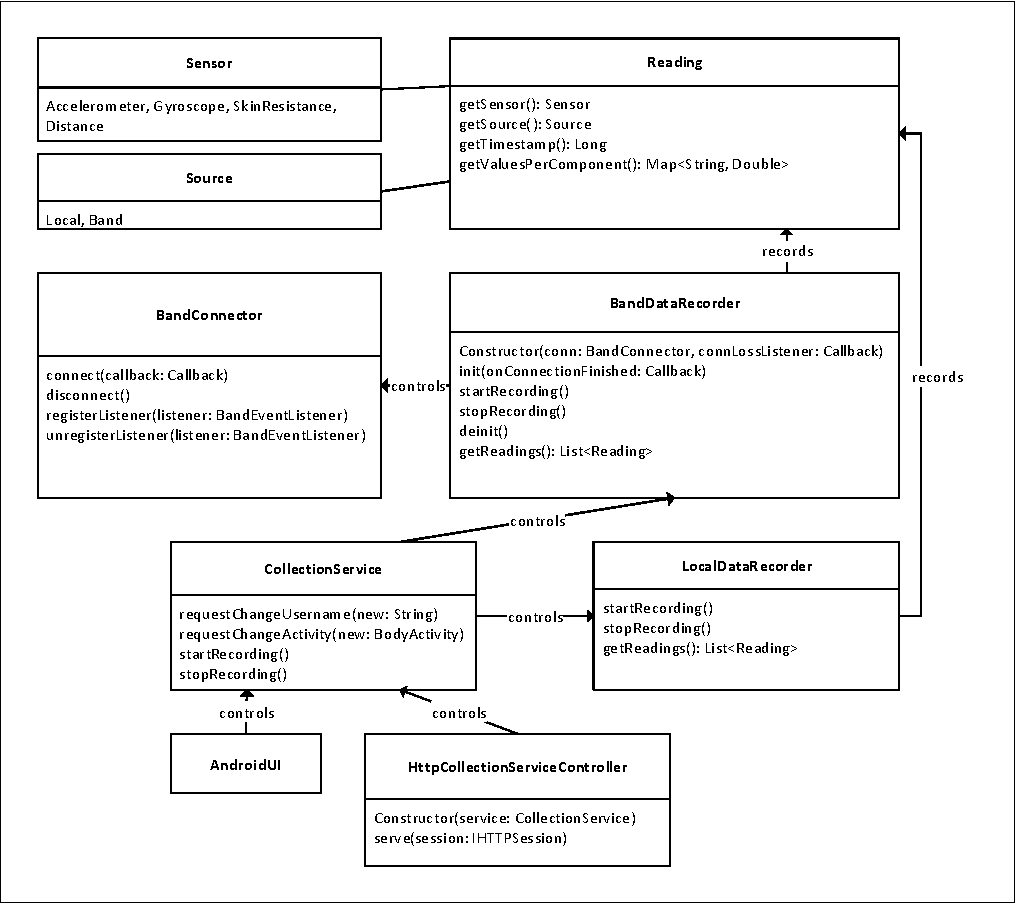
\includegraphics[width=160mm, clip, trim=1mm 1mm 1mm 1mm]{img/app-structure}
\caption{Struktur der Aufzeichnungssoftware}
\label{fig:app-structure}
\end{figure}

Abbildung~\ref{fig:app-structure} bietet einen Überblick über die Struktur der Aufzeichnungssoftware. Im Zentrum steht die Klasse \textit{CollectionService}, die für die robuste Sammlung der Daten verantwortlich ist und daher als persistenter Android-\textit{Service} implementiert ist, der im Gegensatz zu anderen Komponenten einer Android-App nicht ohne weiteres durch das System zur Schonung der Ressourcen beendet werden kann. Gesteuert wird die Aufnahme über eine grafische Benutzeroberfläche auf dem Smartphone selbst (\textit{AndroidUI}), sowie optional auch über eine Weboberfläche, die über einen einfachen HTTP-Server zur Verfügung steht. In den Benutzeroberflächen kann der Name des Probanden, sowie die ausgeführte Aktivität angegeben werden. Des Weiteren wird hierüber die Aufnahme gestartet und gestoppt.

Der \textit{CollectionService} delegiert die Aufnahme an den \textit{BandDataRecorder} und den \textit{LocalDataRecorder} weiter, die jeweils für das Microsoft Band 2 respektive die Smartphone-lokalen Sensoren verantwortlich sind. Über den \textit{BandConnector} wird die Bluetooth-Verbindung zum Band hergestellt und aufrecht erhalten. \textit{BandDataRecorder} und \textit{LocalDataRecorder} zeichnen Daten in Form von \textit{Readings} auf. Die Methode \textit{getValuesPerComponent()} liefert beispielsweise Daten der Form $\{x \to 1.0, y \to 2.0, z \to 3.0\}$, wenn die Komponenten des jeweiligen Sensors der jeweiligen \textit{Source} $\{x, y, z\}$ sind.

Wird die Aufnahme gestoppt, werden die Readings mitsamt den Metadaten Name des Probanden und Aktivität serialisiert und per SFTP auf einen entfernten Speicher hochgeladen. Anschließend werden die Daten von dort abgerufen und wie im folgenden Abschnitt beschrieben weiterverarbeitet.

\section{Transformation der Daten}
\label{sec:transformation}
Jede einzelne Aufnahme eines Nutzers und einer Aktivität besteht aus einer Reihe von Daten mit Zeitstempeln. In dieser Form kann noch kein konventioneller ML-Klassifikationsalgorithmus mit den Daten arbeiten, da diese Daten in Form einer Liste von \textit{Instanzen} erwarten. Eine Instanz besteht aus einer Menge von \textit{Attributen/Features}, die in Rahmen dieser Arbeit bis auf das nominale \textit{Target}-Attribut allesamt kardinal sind. Das Target-Attribut ist dabei die durchgeführte Aktivität. Entsprechend ist eine Transformation der Daten notwendig, um diese tatsächlich nutzbar zu machen.

Um Instanzen zu erzeugen, teilt die Transformationssoftware die Ursprungsdaten zunächst in Intervalle mit zehnsekündiger Dauer auf. Ein solches Intervall soll schließlich eine Instanz, d.h. ein Beispiel für eine Aktivität bilden. Das erste und das letzte Intervall werden gelöscht, da in dieser Zeit die Aufnahme gestartet und gestoppt wurde, was ansonsten durch den anderen Bewegungsablauf die Ergebnisse verfälschen könnte. Aktuell umfasst das Intervall noch mehrere Readings, die aggregiert werden müssen.

\subsection{Beschreibung der Aggregatfunktionen}
Sei $A[1..N]$ eine Liste von Zahlen. Dann seien die folgenden Aggregatfunktionen in Anlehnung an Kwapisz et al.\cite{Kwapisz2011} wie folgt definiert:
\subsubsection{Average}
\[
\text{Avg}(A) := \frac{1}{N} * \sum_{a \in A} a
\]
\subsubsection{Standard Deviation}
\[
\text{StdDev}(A) := \sqrt{\frac{1}{N} * \sum_{a \in A} (a - \text{Avg}(A))^2}
\]
\subsubsection{Average Absolute Difference}
\[
\text{AvgAbsDiff}(A) := \frac{1}{N} * \sum_{a \in A} |\text{Avg}(A) - a|
\]
\subsubsection{$k$-Binned Distribution}
Im Gegensatz zu den obigen Funktionen liefert diese Aggregatfunktion einen $k$-Vektor anstatt einen Skalar. Seien $i \in \{0, ..., k - 1\}, S := \frac{\max A - \min A}{k}$.
\[
\text{Bin}(A, i) := \#\{a \in A | (\min A) + i * S \leq a < (\min A) + (i + 1) * S\}
\]
$\text{Bin}(A, i)$ ist demzufolge die Anzahl der Elemente in Korb $i$, wenn man $A$ der Größe nach sortiert auf $k$ Körbe verteilt. Der Bin ist hierbei als Multimenge zu verstehen und darf somit Elemente auch mehrfach enthalten.
\subsubsection{Average Root of Squares}
Auch diese Aggregatfunktion unterscheidet sich von den bisherigen, da sie mehrere Listen als Parameter erhält:
\[
\text{Aros}(A_1, ..., A_M) = \frac{1}{M} * \sum_{i = 1}^{M} \sqrt{\sum_{a \in A_i} a^2}
\]
\subsubsection{Average Time between Peaks}
Diese Aggregatfunktion gibt die durchschnittliche Zeit zwischen Höhepunkten in $A$ zurück, wofür zusätzlich eine Funktion $\text{timeForIndex}: \mathbb{N} \to \mathbb{N}$ benötigt wird. Die Wahl der Höhepunkte erfolgt durch eine Heuristik. 

Algorithmus~\ref{algo:avgTimeBetweenPeaks} beschreibt die Berechnung des Wertes. Zunächst wird mittels Algorithmus~\ref{algo:indicesOfPeaks} bestimmt, an welchen Indizes in der Liste Werte stehen, die deutlich größer als ihre Nachfolger sind. Dadurch wird definiert, was eine Spitze in dieser spezifischen Liste ausmacht. Anschließend werden Spitzen gesucht, die maximal um den Faktor \textit{threshold} kleiner sind als die größte Spitze, die der Algorithmus gefunden hast. Diese Grenze wird solange gesenkt, bis genügend Spitzen gefunden wurden oder die Grenze so niedrig liegt, dass es sich nicht mehr um Spitzen handelt. Als letztes berechnet der Algorithmus die durchschnittliche Zeit zwischen den Spitzen mithilfe der Funktion \textit{timeForIndex}.

Die im Pseudocode verwendeten Konstanten erwiesen sich im praktischen Test an den gesammelten Daten als gut geeignet. Für andere Datensätze kann eine Anpassung erforderlich sein.

\begin{algorithm}
    \caption{IndicesOfPeaks($A$, $t$), $t \in [0,1]$}
    \label{algo:indicesOfPeaks}
    \Comment{Returns a list of indices $i$ where $A[i] * t \geq A[i+1]$}
    \begin{algorithmic}
        \State $\text{indices} \gets \emptyset$
        \For{$i \in \{1, ..., |A| - 1\}$}
            \If{$A[i] * t \geq A[i+1]$}
                \State $\text{indices} \gets \text{indices} \cup \{i\}$
            \EndIf
        \EndFor
        \State \Return $\text{indices}$
    \end{algorithmic}
\end{algorithm}

\begin{algorithm}
    \caption{AverageTimeBetweenPeaks($A, \text{timeForIndex}, \text{minPeaks}$)}
    \label{algo:avgTimeBetweenPeaks}
    \begin{algorithmic}
        \State \LeftComment \textit{First, heuristically define what a peak is}
        \State $\text{indicesOfPeaks} \gets \text{IndicesOfPeaks}(A, t = 0.8)$
        \If{$\text{indicesOfPeaks} = \emptyset$}
            \State \Return Nil
        \EndIf
        \State $\text{highestPeakIdx} \gets$ Index of highest peak in indicesOfPeaks
        \State \LeftComment{\textit{Lower the threshold until we have found enough peaks or the threshold is too low}}
        \State $\text{otherPeakIndices} \gets \emptyset$
        \State threshold $\gets 0.8$
        \Repeat
            \State otherPeakIndices $\gets$ Indices of $A$ where $A[i] \geq A[\text{highestPeakIdx}] * $ threshold
            \State threshold $\gets \text{threshold} * 0.9$
        \Until{$|\text{otherPeaksIndices}| \geq \text{minPeaks} \vee \text{threshold} < 0.3$}
        \State \LeftComment \textit{Check whether we have found enough peaks}
        \If{$|\text{otherPeakIndices}| < $ minPeaks}
            \State \Return Nil
        \EndIf
        \State \LeftComment \textit{Calculate the average time between the peaks}
        \State timesBetweenPeaks $\gets \emptyset$
        \For{$i \in \{2, ..., |\text{otherPeakIndices}|\}$}
            \State time $\gets$ timeForIndex(otherPeakIndices[$i$]) - timeForIndex(otherPeakIndices[$i - 1$])
            \State timesBetweenPeaks $\gets$ timesBetweenPeaks $\cup \{\text{time}\}$
        \EndFor
        \State \Return \Call{Avg}{timesBetweenPeaks}
    \end{algorithmic}
\end{algorithm}

\subsection{Anwendung der Aggregatfunktionen}
Die Transformationssoftware reduziert nun mithilfe der Aggregatfunktionen die Readings eines jeden Intervalls $I$ auf eine konstante Anzahl skalarer Werte, welche die Features der Instanz darstellen. Im Folgenden sei $I$ ein Array der Struktur $I[G][S][K] \in \mathbb{R}^\alpha$, das die Messungen gruppiert nach Gerät ($G$), Sensor ($S$) und Komponente ($K$) beinhaltet. Des Weiteren sei $F_I$ die Menge der Features des Intervalls $I$. Die Folgenden Unterabschnitte zeigen den Aufbau von $F_I$ mittels der Aggregatfunktionen:
\subsubsection{Pro Kombination von Gerät $G$ und Sensor $S$}
Seien $P$ die einzelnen Komponenten des Sensors, beispielsweise $P = \{x, y, z\}$.
\begin{align*}
    \text{aros} &\gets \text{Aros}(I[G][S][P[1]], ..., I[G][S][P[|P|]]) \\
    F_I &\gets F_I \cup \{((G, S), \text{aros})\}
\end{align*}
Im Kontext betrachtet liefert \textit{Aros} am Beispiel des Beschleunigungssensors gewissermaßen die durchschnittliche Beschleunigung, die alle Achsen zusammen erfahren haben.
\subsubsection{Pro Kombination von Gerät $G$, Sensor $S$ und Komponente $K$}
Sei \textit{timeForIdx} hier eine Funktion, die den Zeitstempel des jeweiligen Datums im Intervall zurückgibt. Sei außerdem $k := 10$, sodass 10 Körbe verwendet werden, was sich experimentell als geeignet herausstellte.
\begin{align*}
    F_I &\gets F_I \cup \{((G, S, K), \text{Avg}(I[G][S][K]))\} \\
    F_I &\gets F_I \cup \{((G, S, K), \text{StdDev}(I[G][S][K]))\} \\
    F_I &\gets F_I \cup \{((G, S, K), \text{AvgAbsDiff}(I[G][S][K]))\} \\
    F_I &\gets F_I \cup \{((G, S, K), \text{AverageTimeBetweenPeaks}(I[G][S][K], \text{timeForIdx}, 3))\} \\
    F_I &\gets F_I \cup \{((G, S, K), \text{Bin}(I[G][S][K], i))\} \forall i \in \{1, ..., k\}
\end{align*}

\subsection{Beispiel}
Wir betrachten für die Aktivität \textit{Jogging} den Beispieldatensatz
\begin{align*}
D = \{&(0, \text{Band}, \text{Gyroscope}, {x \to 1.0, y \to 0.0}), \\
&(0, \text{Band}, \text{Accelerometer}, {x \to 1.0, y \to 1.0}), \\
&(1000, \text{Band}, \text{Gyroscope}, {x \to 2.0, y \to 2.0}), \\
&(1000, \text{Band}, \text{Accelerometer}, {x \to 0.0, y \to 1.0}), \\
&(2000, \text{Band}, \text{Gyroscope}, {x \to 3.0, y \to 0.0}), \\
&(2000, \text{Band}, \text{Accelerometer}, {x \to 1.0, y \to 3.0})\}
\end{align*} 

Zur Vereinfachung wird von 2D-Sensoren ausgegangen, sodass keine $z$-Komponente vorhanden ist. Zur werden als Aggregatfunktionen der Durchschnitt, die \textit{Binned Distribution} mit zwei \textit{Bins} und der \textit{Average Root of Squares} verwendet. Die gewählte Intervallgröße beträgt zwei Sekunden, sodass sich die folgenden Intervalle ergeben:
\begin{align*}
I_1 = \{&(0, \text{Band}, \text{Gyroscope}, {x \to 1.0, y \to 0.0}), \\
&(0, \text{Band}, \text{Accelerometer}, {x \to 1.0, y \to 1.0}), \\
&(1000, \text{Band}, \text{Gyroscope}, {x \to 2.0, y \to 2.0}), \\
&(1000, \text{Band}, \text{Accelerometer}, {x \to 0.0, y \to 1.0})\},
\end{align*}
\begin{align*}
I_2 = \{&(2000, \text{Band}, \text{Gyroscope}, {x \to 3.0, y \to 0.0}), \\
&(2000, \text{Band}, \text{Accelerometer}, {x \to 1.0, y \to 3.0})\}
\end{align*}
Nun werden die Aggregatfunktionen auf $I_1$ angewendet:
\begin{align*}
&\text{Avg}_\text{Band, Gyroscope, x} = (1 + 2)/2 = 1.5 \\
&\text{Avg}_\text{Band, Gyroscope, y} = (0 + 2)/2 = 1 \\
&\text{Avg}_\text{Band, Accelerometer, x} = (1 + 0)/2 = 0.5 \\
&\text{Avg}_\text{Band, Accelerometer, y} = (1 + 1)/2 = 1 \\
&\text{Bin}_\text{Band, Gyroscope, x}(0) = \#\{1\} = 1 \\
&\text{Bin}_\text{Band, Gyroscope, x}(1) = \#\{2\} = 1 \\
&\text{Bin}_\text{Band, Gyroscope, y}(0) = \#\{0\} = 1 \\
&\text{Bin}_\text{Band, Gyroscope, y}(1) = \#\{2\} = 1 \\
&\text{Bin}_\text{Band, Accelerometer, x}(0) = \#\{0\} = 1 \\
&\text{Bin}_\text{Band, Accelerometer, x}(1) = \#\{1\} = 1 \\
&\text{Bin}_\text{Band, Accelerometer, y}(0) = \#\{0\} = 0 \\
&\text{Bin}_\text{Band, Accelerometer, y}(1) = \#\{1\} = 0 \\
&\text{Aros}_\text{Band, Gyroscope} = (1/2) * (\underbrace{\sqrt{1^2 + 2^2}}_x + \underbrace{\sqrt{0^2 + 2^2}}_y) \approx 2.12 \\
&\text{Aros}_\text{Band, Accelerometer} = (1/2) * (\underbrace{\sqrt{1^2 + 0^2}}_x + \underbrace{\sqrt{1^2 + 1^2}}_y) \approx 1.2 \\
\end{align*}
Die Berechnung für $I_2$ erfolgt analog. Aus den obigen Features ergibt sich der folgende Datensatz, der von einem herkömmmlichen Klassifikationsalgorithmus verarbeitet werden kann:\\

\begin{tabular}{|c|c|c|c|c|c|c|c|c|c|c|c|c|c|c|c|}
	\hline 
	Intervall & $\text{Avg}_\text{Band, Gyroscope, x}$ & $\text{Avg}_\text{Band, Gyroscope, y}$  & $...$  & sampleClass  \\ 
	\hline 
	$I_1$ & $1.5$ & $1$ & $...$ & Jogging \\ 
	\hline 
	$I_2$ & $...$ & $...$ & $...$ & Jogging   \\ 
	\hline 
\end{tabular} \\

Die Intervallspalte dient nur der Illustration.

\subsection{Nachbearbeitung der Daten}
Bei der Transformation kann sich das Problem ergeben, dass nicht jede Zelle der resultierenden Tabelle einen Wert enthält. Dazu kann es beispielsweise kommen, wenn der Algorithmus \texttt{AverageTimeBetweenPeaks} \textit{Nil} zurückgibt. Enthält eine Zelle keinen Wert, so wird in ihr der Durchschnittswert des gefüllten Teils der Spalte eingesetzt. Um dem Risiko vorzubeugen, dass ML-Algorithmen Spalten mit betragsmäßig hohen Werten fälschlicherweise auch automatish hohen Einfluss zuschreiben, werden alle numerischen Spalten mithilfe des z-Score-Verfahrens normalisiert. Dazu wird von den Werten jeder Spalte der Durchschnittswert dieser abgezogen, wonach das Resultat durch die Standardabweichung der Spalte geteilt wird. Der Betrag einer Zelle gibt dann an, wie viele Standardabweichungen vom Durchschnitt abgewichen wird.  

\section{Anwendung von ML-Klassifikationsalgorithmen}
\label{section:ml-algos}
Um die Vergleichbarkeit mit \cite{Weiss2016} sicherzustellen, wurde die Java-basierte ML-Software WEKA zum maschinellen Lernen verwendet. Diese bietet fertige Implementierungen diverser ML-Algorithmen an, die sowohl mittels einer grafischen Benutzeroberfläche, als auch in Code verwendet werden können. Die in dieser Arbeit verwendeten Algorithmen entsprechen denen aus \cite{Weiss2016} und werden im Folgenden kurz beschrieben. Falls nicht anders angegeben, wurden für jedes Modell die standardmäßigen Hyperparameter verwendet. Dabei handelt es sich um Parameter, die der jeweilige Algorithmus nicht selbst lernen kann.
\todo{Hyperparameter aktualisieren, falls nötig}
\subsection{Random Forest (RF)}
Ein \textit{Random Forest} ist ein Wald von Entscheidungsbäumen (erklärt in Kapitel 14.4 \cite{Bishop2006}), die randomisiert entstanden sind. Soll eine neue Instanz klassifiziert werden, treffen alle Entscheidungsbäume eine Entscheidung und die am häufigsten vorhergesagte Klasse gewinnt. WEKA nutzt eine Implementierung nach \cite{Breiman2001}. Experimentell haben sich die folgenden Hyperparameterwerte als sinnvoll erwiesen: Die Anzahl der Bäume in Wald wurde auf 50, die Anzahl der verwendeten Features pro Baum auf 10, sowie die maximale Tiefe auf 25 festgelegt.
\subsection{J48-Entscheidungsbaum (J48)}
J48 ist eine Implementierung des \textit{C4.5}-Algorithmus\cite{Quinlan1993}. Der Entscheidungsbaum wird anhand von Trainingsdaten $T$ iterativ durch das Hinzufügen von Entscheidungsknoten erzeugt, die den Informationsgehalt der Teilmengen von $T$ minimieren, die aus dem Split an jenem Entscheidungsknoten hervorgehen. Der Informationsgehalt umso höher, je mehr verschiedene Klassen sich in einer Menge von Instanzen befinden. Ein niedriger Informationsgehalt besagt demnach, dass nach einer Entscheidung an einem Entscheidungsknoten klarer geworden ist, welcher Klasse die Instanzen in den Mengen nach dem Split zuzuordnen sind.
\subsection{Instance-Based-Learner (IB$k$)}
Der IB$k$-Algorithmus ist ein $k$NN-basierter Klassifikationsalgorithmus. Soll einer neuen Instanz $x \in \mathbb{R}^n$ eine Klasse zugeordnet werden, werden anhand eines Distanzmaßes für den Vektorraum $\mathbb{R}^n$ die $k$ nächsten Nachbarn von $x$ gesucht. $x$ wird danach die Klasse zugeordnet, die unter den $k$ Nachbarn am häufigsten vorkam. Weitere Details sind zu finden in \cite{Aha1991}.
$k$ ist dabei ein Hyperparameter, der auf 3 eingestellt wurde.
\subsection{Naive Bayes (NB)}
Naive Bayes ist eine probabilistische Methode zur Klassifikation\cite{John1995}. Mit $x = (x_1, ..., x_n)$ wird die Klasse $C$ gesucht, die $\mathbb{P}(C | x_1, ..., x_n)$ maximiert. $x$ besteht hier aus nominalen Attributen. Der Satz von Bayes besagt, dass $\mathbb{P}(C|x) = \frac{\mathbb{P}(C) \mathbb{P}(x | C)}{\mathbb{P}(x)}$. Da über $C$ optimiert wird, kann der Nenner für diesen Ansatz ignoriert werden. Nimmt man \textit{naiv} an, dass $x_1, ..., x_n$ voneinander unabhängig sind, kann somit statt $\mathbb{P}(C | x)$ auch folgender Term über $C$ maximiert werden: $\mathbb{P}(C) \prod_{i=1}^{n} \mathbb{P}(x_i | C)$. Durch den Trainingsdatensatz sind $\mathbb{P}(C)$ als Prior der Klasse $C$, sowie alle $\mathbb{P}(x_i | C)$ bekannt, sodass der Term durch einfaches Ausprobieren aller Klassen maximiert werden kann.

Enthält $x$ numerische Attribute, müssen diese zunächst durch nominale Attribute ersetzt werden. Der Wertebereich aller $x_i$ über den Trainingsdatensatz hinweg kann in eine feste Anzahl von Intervallen aufgeteilt werden. Für jedes Intervall $I$ wird nun eine Indikatorvariable als Feature angelegt, die angibt, ob für eine Instanz $x$ gilt, dass $x_i \in I$.
\subsection{Multilayer Perceptron (MLP)}
Bei dieser Methode handelt es sich um ein mehrschichtiges Netzwerk von sogenannten \textit{Perzeptren}, auch \textit{(künstliches) neuronales Netzwerk} genannt. Ein Perzeptron erhält $n$ Eingaben $x_1, ..., x_n$ und gewichtet diese mit Parametern $\Theta_1, ..., \Theta_n$, die gelernt werden. Das Perzeptron berechnet $y = g(\sum_{i=1}^{n} \Theta_i x_i)$ als Ausgabewert, wobei $g$ eine Aktivierungsfunktion ist, die den Ausgabewerte beschränkt, beispielsweise die Sigmoidfunktion.

Die Ausgabe eines Perzeptron kann einem Perzeptron der nächsten Schicht als Eingang dienen. Die letzte Schicht fungiert als Ausgabe des Netzwerks, dessen Fehler anhand eines Trainingsdatensatzes bestimmt werden kann. Jedes Perzeptron berechnet, wie die eigenen Parameter $\Theta$ angepasst werden müssen, um den Fehler zu minimieren, wofür der Fehler der Perzeptren der letzten Schicht an die vorherige Schicht weiter propagiert wird (\textit{Backpropagation}). Zur Optimierung der Parameter wird ein stochastischer Gradientenabstieg verwendet. Zur Klassifikation können die Ausgangswerte der Perzeptren der letzten Schicht als Indikatorvariablen für die vorhandenen Klassen interpretiert werden. Weitere Informationen sind zu finden in \cite{Haykin1994}.